\section{Einleitung}
\subsection{Motivation}
%
%
\begin{frame}
	\frametitle{Überblick}
	\tableofcontents[currentsubsection]
\end{frame}
%
%
\begin{frame}
		\frametitle{Motivation - Kleine und große Katastrophen (1)}
	\begin{columns}
		\begin{column}{0.48\textwidth}
			\begin{figure}
				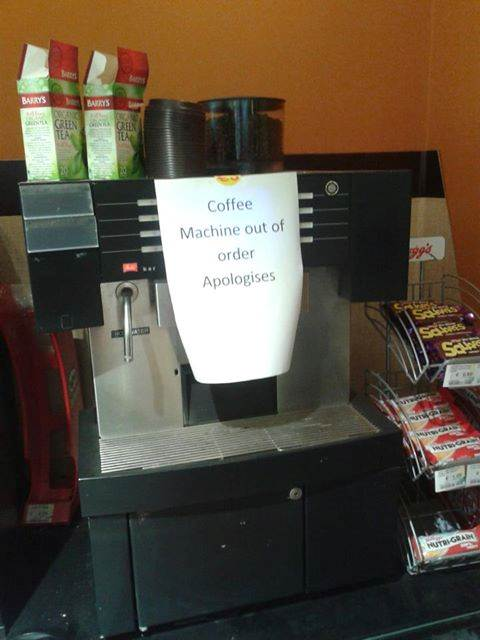
\includegraphics[scale=0.36]{grafiken/broken2}		
				\caption{Defekte Kaffeemaschine
					\footnotemark	
				}		
			\end{figure}
		\end{column}
		\begin{column}{0.48\textwidth}
			Kleine Katastrophe:
			\begin{itemize}
				\item Kaffeemaschine defekt
				\item Folge: Müder Informatiker
			\end{itemize}
		\end{column}		
	\end{columns}
	\footnotetext{Quelle: \url{https://jlonerga.wordpress.com}}
\end{frame}
%
%
\begin{frame}
	\frametitle{Motivation -  Kleine und große Katastrophen (2)}
	\begin{columns}
		\begin{column}{0.48\textwidth}
			\begin{figure}
				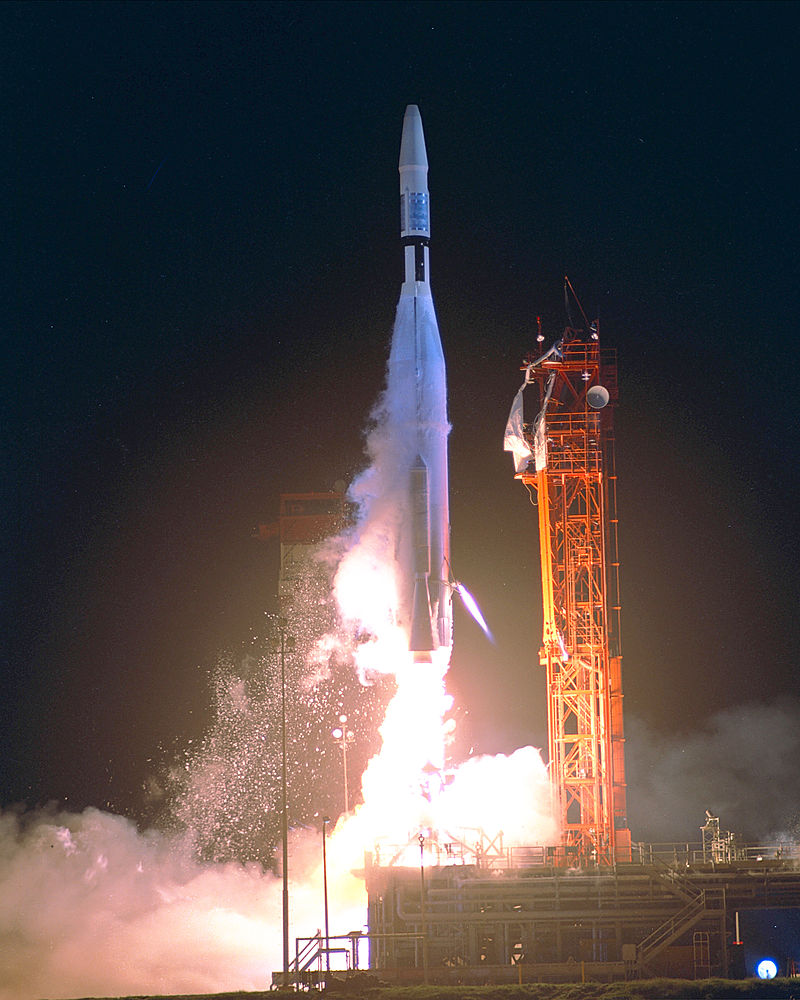
\includegraphics[scale=0.6]{grafiken/mariner}		
				\caption{Fehlerhafte Trägerrakete
					\footnotemark		
				}		
			\end{figure}
		\end{column}
		\begin{column}{0.48\textwidth}
			Große Katastrophe:
			\begin{itemize}
				\item Start der Trägerrakete der Raumsonde \emph{Mariner 1} (1962)
				\pause
				\item Missverständnis beim Implementieren der Spezifikation
				\pause
				\item Folgen:
				\begin{itemize}
					\item Rohe- anstatt geglättete Messdaten
					\item Starke Abweichung vom Kurs
					\item Notsprengung der Rakete nach ca. 5 Minuten
					\item Schaden von ca. 18,5 Millionen Dollar
				\end{itemize}
			\end{itemize}
		\end{column}
		
	\end{columns}
	\footnotetext{Quelle: \url{NASA}}
\end{frame}
%
%
%
\begin{frame}
	\frametitle{Motivation - Lösung für kleine Katastrophen}
	\begin{figure}
		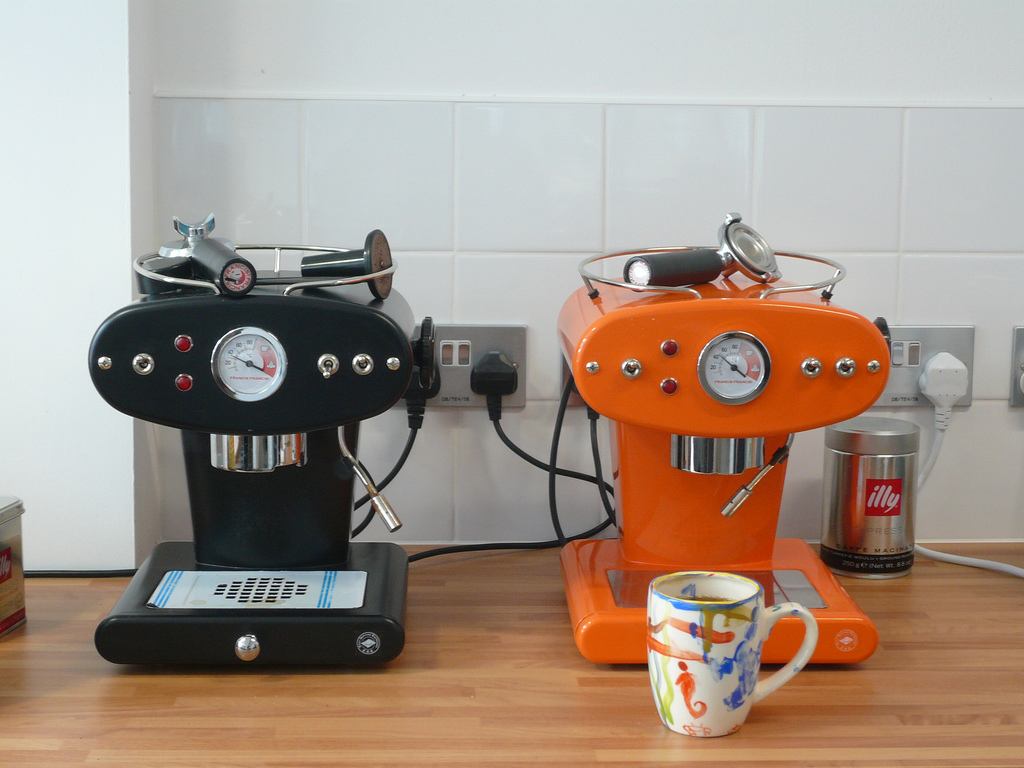
\includegraphics[scale=0.2]{grafiken/working}		
		\caption{Ansatz - Doppelt hält besser
			\footnote{\tiny Quelle: \url{http://www.sarahmei.com} }
		}		
	\end{figure}
\end{frame}
%
%
%
\begin{frame}
	\frametitle{Motivation - Lösung für große Katastrophen}

	\begin{center}
		{\huge So ähnlich?}
	\end{center}
\end{frame}
%
%
%
\subsection{Ansätze für zuverlässige Systeme}
%
\begin{frame}
	\frametitle{Ansätze für zuverlässige Systeme}
	Zwei unterschiedliche Ansätze für zuverlässige Software-Systeme:
		
		\begin{itemize}
			\pause
			\item Präventiver Ansatz
			\begin{itemize}
				\item Ziel: Eliminierung alle Programmfehler vor produktivem Einsatz
				\item Verwendung von Hochsprachen
				\item Testgetriebene Entwicklung
				\item Testautomatisierung	
			\end{itemize}
			\pause	
			\item Fehlertoleranz im laufenden Betrieb	
			\begin{itemize}
				\item Fehlerentdeckung und -behandlung
				\item Fehlertolerante Algorithmen
				\item Recovery-Blocks
				\item N-Version Programmierung
			\end{itemize}
			
		\end{itemize}	
\end{frame}
%
%
\begin{frame}
	\frametitle{Überblick}
	\tableofcontents[currentsubsection]
\end{frame}
%
%
\begin{frame}
	\frametitle{Ansätze für zuverlässige Systeme - Historischer Gedanke}
	\begin{block}{Idee der redundanten Berechnung von Ergebnissen \cite{lardner}}
		\enquote{\emph{The most certain and effectual check upon errors which arise in the process of computation,	is to cause the same computations to be made by separate and independent computers; and this	check is rendered still more decisive if they make their computations by different methods.}}
	\end{block}
\end{frame}
%
%
\begin{frame}
	\frametitle{Ansätze für zuverlässige Systeme - Recovery Blocks (1)}
	Erster Ansatz redundanter Berechnungen in Software: Recovery Blocks \cite{Horning:1974:PSE:647641.733522}
	\begin{figure}
		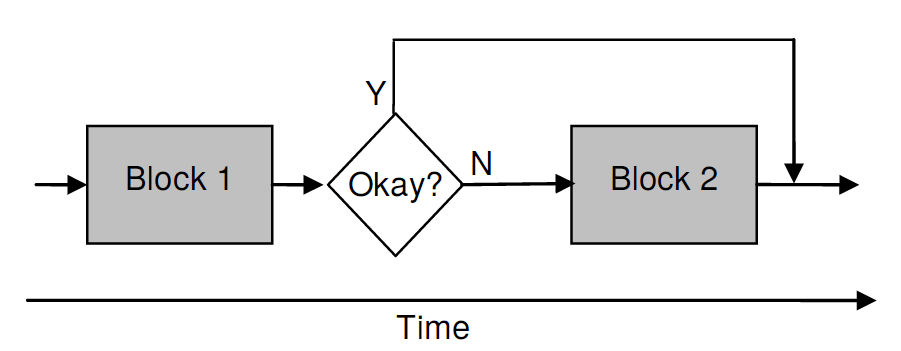
\includegraphics[scale=0.3]{grafiken/recovery-block.png}		
		\caption{Ansatz der Recovery-Blocks
			\footnotemark		
		}		
	\end{figure}
	\footnotetext{Quelle: \cite{lucent}}
\end{frame}
%
%
\begin{frame}
	\frametitle{Ansätze für zuverlässige Systeme - Recovery Blocks (2)}
	Eigenschaften:
	\begin{itemize}
		\item Akzeptanztest teilweise so aufwendig wie die eigentliche Funktionalität 
		\item Zeitliche Verzögerung im Falle eines fehlgeschlagenen Tests
	\end{itemize}	
\end{frame}